\documentclass[a4paper, norsk, 12pt]{article}
\usepackage{babel,textcomp}
\usepackage[norsk]{isodate}
\usepackage[utf8]{inputenc}
\usepackage[T1]{fontenc}
\usepackage{listingsutf8}
\usepackage{graphicx}
\usepackage{amsmath,scalerel}
\usepackage{fancyhdr}
\usepackage{enumitem}
\usepackage{paralist}
\usepackage{dsfont}
\usepackage{upgreek}
\usepackage[usenames, dvipsnames]{color}
\usepackage{subcaption}
\usepackage{float}
\usepackage{graphicx}



\definecolor{dkgreen}{rgb}{0,0.6,0}
\definecolor{gray}{rgb}{0.5,0.5,0.5}
\definecolor{mauve}{rgb}{0.58,0,0.82}


\lstset{frame=tb,
  language=matlab,
  aboveskip=3mm,
  belowskip=3mm,
  showstringspaces=false,
  columns=flexible,
  basicstyle={\small\ttfamily},
  numbers=none,
  numberstyle=\tiny\color{gray},
  keywordstyle=\color{blue},
  commentstyle=\color{dkgreen},
  stringstyle=\color{mauve},
  breaklines=true,
  breakatwhitespace=true,
  tabsize=3,
  inputencoding=ansinew,
  extendedchars=true,
  literate={æ}{{\ae}}1 {å}{{\aa}}1 {ø}{{\o}}1 {Æ}{{\AE}}1 {Å}{{\AA}}1 {Ø}{{\O}}1,
}

\pagestyle{fancy}
\fancyhf{}
\rhead{21.09.2018}
\chead{INF4490 REPORT}
\lhead{William Arild Dahl}
\rfoot{\thepage}
\makeatletter
\setlength{\@fptop}{0pt}
\makeatother
\parfillskip=3em plus1fil

\begin{document}
\begin{titlepage}

\newcommand{\HRule}{\rule{\linewidth}{0.5mm}} % Defines a new command for the horizontal lines, change thickness here

\center % Center everything on the page

%----------------------------------------------------------------------------------------
%	HEADING SECTIONS
%----------------------------------------------------------------------------------------

\textsc{\LARGE Universitetet i Oslo}\\[1.5cm] % Name of your university/college
\textsc{\Large INF4490}\\[0.5cm] % Major heading such as course name
\textsc{\large Biologically inspired computing}\\[0.5cm] % Minor heading such as course title

%----------------------------------------------------------------------------------------
%	TITLE SECTION
%----------------------------------------------------------------------------------------

\HRule \\[0.4cm]
{ \huge \bfseries Traveling Salesman Problem}\\[0.4cm] % Title of your document
\HRule \\[1.5cm]


%----------------------------------------------------------------------------------------
%	AUTHOR SECTION
%----------------------------------------------------------------------------------------

%\begin{minipage}{0.4\textwidth}
%\begin{flushleft} \large
%\emph{Author:}\\
%John \textsc{Smith} % Your name
%\end{flushleft}
%\end{minipage}
%~
%\begin{minipage}{0.4\textwidth}
%\begin{flushright} \large
%\emph{Supervisor:} \\
%Dr. James \textsc{Smith} % Supervisor's Name
%\end{flushright}
%\end{minipage}\\[2cm]

% If you don't want a supervisor, uncomment the two lines below and remove the section above
\Large

William Arild Dahl\\ % Your name
\textsc{Username:} williada\\[3cm]



%----------------------------------------------------------------------------------------
%	DATE SECTION
%----------------------------------------------------------------------------------------

{\large 21.09.2018}\\[2cm] % Date, change the \today to a set date if you want to be precise

%----------------------------------------------------------------------------------------
%	LOGO SECTION
%----------------------------------------------------------------------------------------


\includegraphics[width=1\textwidth]{uio_banner.png}\\[1cm] % Include a department/university logo - this will require the graphicx package

%----------------------------------------------------------------------------------------

\vfill % Fill the rest of the page with whitespace
\end{titlepage}

%------------------------------------------------------------------------------
%               Text section
%------------------------------------------------------------------------------

\section{Introduction}

In this assignment, we were expected to solve the Traveling Salesman Problem using brute force, simple stochasticism and genetic algorithms. All code is written in Python (3.6.4). 
I chose to keep each part of the assignment contained in one python script, and created a \texttt{functions.py} for methods that are used by all scripts. Here is how to run any script:\newline\newline 
	\begin{lstlisting}
	python3 ./<script.py>
	
	\end{lstlisting}

All simulations are run on a Intel Core m5-6Y54 CPU @ 1.10GHz.
 

\section{Exhaustive Search}
Brute force a very simple approach to the TSP, and in my case, the only solution i knew about before starting this course. It explores every possible tour and is therefore guaranteed to find the optimal solution. Exhaustive search, also called Brute Force has a \textbf{very} high complexity: $\mathcal{O}{n!}$ with $n$ being the number of cities. 
\newline \newline 
Running exhaustive search with 6-10 cities produced the following results: 
	\begin{lstlisting}
	Runtime for 6 cities is: 0.00172 seconds.
	Minimum distance is: 5018.81.
	
	Runtime for 7 cities is: 0.01516 seconds.
	Minimum distance is: 5487.89.
		
	Runtime for 8 cities is: 0.13097 seconds.
	Minimum distance is: 6667.49.
	
	Runtime for 9 cities is: 1.23250 seconds.
	Minimum distance is: 6678.55.

	Runtime for 10 cities is: 14.47876 seconds.
	Minimum distance is: 7486.31.

	Shortest tour for 10 cities:
	['Copenhagen', 'Hamburg', 'Brussels', 'Dublin', 'Barcelona', 'Belgrade', 'Istanbul', 'Bucharest', 'Budapest', 'Berlin']
	\end{lstlisting}
As we can see, the runtime increases dramatically with each added city to the problem, this is due to the factorial complexity of the algorithm.I am estimating that my CPU can check somewhere in the range of 250,000 - 280,000 permutations/second. 
\[ 
	t =  \frac{n!}{p}
\]
Where $t$ is time in seconds , $n$ is the number of cities, and $p$ is the number of permutations/second. 
If I were to run my code with 24 cities we are looking at a runtime of about $4.4\times 10^{12}$ years\footnote{318 times longer than the universe has existed.}.

\section{Hill Climbing}
Hill Climbing is a stochastic method. I solved it by choosing a random starting point(permutation) and calculating its tour length. I then swap two random genes in the genome and calculate this genomes tour length. I repeat this random swapping 1000 times and always keep the better result. This way the algorithm is 'climbing' up towards a local optima, or preferably a global optima if I am lucky. Hill Climbing is greedy, so it will only and will always pick the better neighbor. That means that there is a great possibility that the algorithm will end up in a local optima. I choose to use 20 random starting points to ensure more exploring.
\newline\newline
Here are the results of 20 random starting points and 1000 gene swaps: 
	\begin{lstlisting}
	Runtime for 10 cities visited: 0.1891 seconds.
	Length of best tour is: 7486.31.
 	Length of worst tour is: 8377.24.
 	Length of average tour is: 7652.89.
 	Standard deviation is: 261.32. 
 	Route of best tour is:['Copenhagen', 'Hamburg', 'Brussels', 'Dublin', 'Barcelona', 'Belgrade', 'Istanbul', 'Bucharest', 'Budapest', 'Berlin'].

	Runtime for 24 cities visited: 0.2843 seconds. 
	Length of best tour is: 12967.29.
 	Length of worst tour is: 17152.05.
 	Length of average tour is: 14917.95.
 	Standard deviation is: 1183.94. 
 	Route of best tour is:['London', 'Paris', 'Brussels', 'Prague', 'Vienna', 'Budapest', 'Bucharest', 'Istanbul', 'Sofia', 'Belgrade', 'Warsaw', 'Kiev', 'Moscow', 'Saint Petersburg', 'Stockholm', 'Copenhagen', 'Hamburg', 'Berlin', 'Munich', 'Milan', 'Rome', 'Barcelona', 'Madrid', 'Dublin'].
	\end{lstlisting}
	As we can see the algorithm is significantly faster than exhaustive search. In this run for $N = 10$, hill climbing was able to find the global optima, which is confirmed by exhaustive search. However, this is not always the case for every run, but the algorithm gets fairy close every time. We can also observe that the increase to $N = 24$ did not impact the runtime significantly. I am fairly sure that the tour for 24 cities is \textbf{not} the global optima, but considering the runtime of an exhaustive search, the answer is probably good enough.   

\section{Genetic Algorithm}

For the genetic algorithm I have followed the procedure described in class. First initialize a random population, do a selection of parents, crossover to create children, mutate children with a mutation rate, and finally do a survivor selection.
\newline\newline
I choose to do Partially Mapped Crossover for recombination. I believe this is a good choice since we are dealing with permutations where adjacency is important. For choosing which parents get to mate, I choose a random selection of 10 \% of existing parents to compete with each other for mating. The two best are chosen based on their distance. This is done until new population is filled up with a new generation. I also save the best individual of each generation no matter what. Since this limits the exploration a bit, I choose to save a random selection (5\%) of previous generation to live on. 
\newline\newline
For mutation i choose inversion mutation. This saves adjacency a bit, but also stimulates more exploration. My mutation rate is initially set to 0.05, but changes to 0.025 for the last 20\% generations. As the generations run, we will in theory have a more homogeneous population, approaching a optima, so there is no reason to mutate as much for later generations.
\newline\newline
Here are the results:
	\begin{lstlisting}
	10 cities, with 50 population and 50 generations:
	Length best tour: 7486.31.
 	Length of worst tour: 13082.20.
 	Length of average tour: 7851.31.
 	Standard deviation is: 318.16651293140956.
	Route of the best tour is: ['Hamburg', 'Brussels', 'Dublin', 'Barcelona', 'Belgrade', 'Istanbul', 'Bucharest', 'Budapest', 'Berlin', 'Copenhagen']
 	Searched 50980 routes.
 	Runtime: 2.0367


	10 cities, with 100 population and 50 generations:
 	Length best tour: 7486.31.
 	Length of worst tour: 11318.40.
 	Length of average tour: 7690.10.
 	Standard deviation is: 324.77759470178034.
 	Route of the best tour is: ['Brussels', 'Dublin', 'Barcelona', 'Belgrade', 'Istanbul', 'Bucharest', 'Budapest', 'Berlin', 'Copenhagen', 'Hamburg']
 	Searched 100000 routes.
 	Runtime: 5.4033


	10 cities, with 150 population and 50 generations:
	Length best tour: 7486.31.
 	Length of worst tour: 12735.37.
 	Length of average tour: 7633.63.
	Standard deviation is: 346.77838812167613.
 	Route of the best tour is: ['Hamburg', 'Brussels', 'Dublin', 'Barcelona', 'Belgrade', 'Istanbul', 'Bucharest', 'Budapest', 'Berlin', 'Copenhagen']
 	Searched 150000 routes.
 	Runtime: 12.0743



 	24 cities, with 100 population and 100 generations:
 	Length best tour: 15031.78.
 	Length of worst tour: 20365.55.
	Length of average tour: 16798.05.
	Standard deviation is: 210.95537216591538.
 	Route of the best tour is: ['Budapest', 'Warsaw', 'Copenhagen', 'Stockholm', 'Saint Petersburg', 'Moscow', 'Kiev', 'Belgrade', 'Istanbul', 'Bucharest', 'Sofia', 'Rome', 'Prague', 'Hamburg', 'Berlin', 'Paris', 'London', 'Dublin', 'Brussels', 'Barcelona', 'Madrid', 'Milan', 'Munich', 'Vienna']
 	Searched 200000 routes.
 	Runtime: 21.9051


	24 cities, with 200 population and 100 generations:
 	Length best tour: 13967.29.
 	Length of worst tour: 20597.20.
 	Length of average tour: 16149.77.
 	Standard deviation is: 331.58758263762104.
	Route of the best tour is: ['Munich', 'Hamburg', 'Copenhagen', 'Berlin', 'Prague', 'London', 'Dublin', 'Brussels', 'Paris', 'Madrid', 'Barcelona', 'Rome', 'Milan', 'Belgrade', 'Sofia', 'Bucharest', 'Istanbul', 'Kiev', 'Moscow', 'Saint Petersburg', 'Stockholm', 'Warsaw', 'Budapest', 'Vienna']
 	Searched 401980 routes.
 	Runtime: 82.0477


	24 cities, with 300 population and 100 generations:
 	Length best tour: 13145.62.
 	Length of worst tour: 21199.85.
 	Length of average tour: 15329.09.
	Standard deviation is: 325.9959758299527.
 	Route of the best tour is: ['Hamburg', 'Copenhagen', 'Stockholm', 'Warsaw', 'Saint Petersburg', 'Moscow', 'Kiev', 'Bucharest', 'Istanbul', 'Sofia', 'Belgrade', 'Rome', 'Milan', 'Barcelona', 'Madrid', 'Dublin', 'London', 'Paris', 'Brussels', 'Munich', 'Vienna', 'Budapest', 'Prague', 'Berlin']
 	Searched 600000 routes.
 	Runtime: 166.3824

	\end{lstlisting}
As we can see from the runs with 10 cities, all population sizes gives us the correct shortest route. Compared to pure Hill Climbing it is quite a bit slower, and the runtime increases as expected for larger population pools. Standard deviation stay about the same for all three population sizes which is a bit surprising, as I expected it to be a bit higher for a larger population. the GA is however \textbf(much) faster than exhaustive search since it does fewer route searches.\newline\newline\newline\newline
When we examine the the GA for 24 cities we can see that the length of best solution does not change much from 200 population to 300 population, while runtime is doubled. There is no way for us to verify the answer the three runs produces, but since we are lowering the shortest distance by such a small margin, we can assume we are approaching an acceptable optima. Below are the plots for average fitness through generations for the different populations for 10 and 24 cities:
	\begin{figure}[h!]
	\centering
	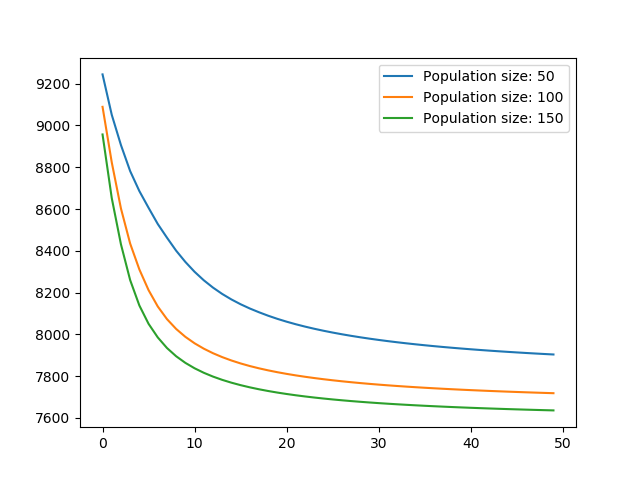
\includegraphics[width=1.0\textwidth]{ga_plt_10.png}
	\end{figure}
\newpage
	\begin{figure}[t!]
	\centering
	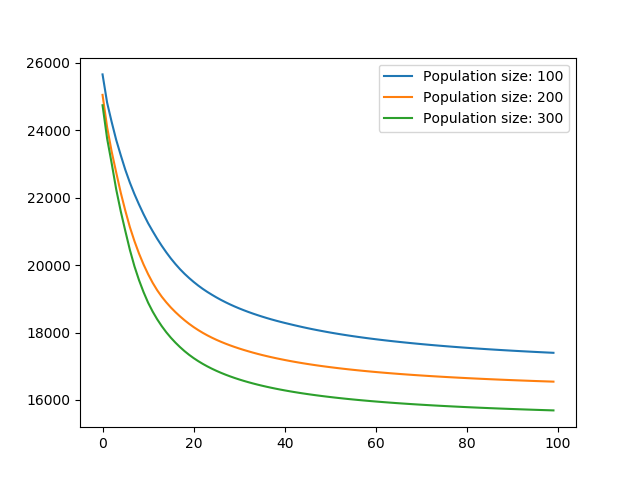
\includegraphics[width=1.0\textwidth]{ga_plt_24.png}
	\end{figure}
For both city numbers, it seems like both benefit from having a larger population size, however the difference is greater for 24 cities than for 10 cities. For both of them, the larger population helps us get a better average fitness across generations, which makes sense. Especially for the first generation, there is a big difference in fitness. 

\section{Hybrid Algorithm}

The hybrid algorithm is implemented as described in the lecture. For each round of parent selection I run each parent for 5 iterations of Hill Climbing, to boost their fitness. As described in the lecture, for the $Lamarckian$ model we use the improved genome for crossover and mutation, while for the $Baldwinian$ model the original genome is used. For both models, the new fitness created by Hill Climbing is used to determine which 2 parents of the random parent pool gets to mate. I choose to go test both models with the average population numbers from the Genetic Algorithm. So for 10 cities I used a population size of 50, and ran it for 50 generations. For 24 cities I used a population size of 100 and ran it for 100 generations. Here are the results:\newline\newline 
	\begin{lstlisting}
	Lamarckian: 10 cities, with 50 population and 50 generations:
 	Length best tour: 7486.31.
  	Length of worst tour: 10304.37.
  	Length of average tour: 7528.05.
  	Standard deviation is: 219.28808361532802.
  	Route of the best tour is: ['Copenhagen', 'Hamburg', 'Brussels', 'Dublin', 'Barcelona', 'Belgrade', 'Istanbul', 'Bucharest', 'Budapest', 'Berlin']
  	Searched 50980 routes.
  	Runtime: 9.5032


 	Baldwinian: 10 cities, with 50 population and 50 generations:
  	Length best tour: 7486.31.
  	Length of worst tour: 10304.37.
  	Length of average tour: 7548.83.
  	Standard deviation is: 320.78448135236073.
  	Route of the best tour is: ['Copenhagen', 'Hamburg', 'Brussels', 'Dublin', 'Barcelona', 'Belgrade', 'Istanbul', 'Bucharest', 'Budapest', 'Berlin']
  	Searched 50980 routes.
  	Runtime: 11.4831


 	Lamarckian: 24 cities, with 100 population and 100 generations:
 	Length best tour: 12287.07.
    Length of worst tour: 17728.28.
    Length of average tour: 12806.01.
  	Standard deviation is: 413.3071816662872.
  	Route of the best tour is: ['Budapest', 'Vienna', 'Warsaw', 'Berlin', 'Prague', 'Munich', 'Milan', 'Rome', 'Barcelona', 'Madrid', 'Dublin', 'London', 'Paris', 'Brussels', 'Hamburg', 'Copenhagen', 'Stockholm', 'Saint Petersburg', 'Moscow', 'Kiev', 'Bucharest', 'Istanbul', 'Sofia', 'Belgrade']
  	Searched 200000 routes.
  	Runtime: 139.8681


 	Baldwinian: 24 cities, with 100 population and 100 generations:
  	Length best tour: 12325.93.
  	Length of worst tour: 17260.79.
  	Length of average tour: 12864.27.
  	Standard deviation is: 393.46614619400503.
  	Route of the best tour is: ['Warsaw', 'Vienna', 'Budapest', 'Belgrade', 'Sofia', 'Istanbul', 'Bucharest', 'Kiev', 'Moscow', 'Saint Petersburg', 'Stockholm', 'Copenhagen', 'Berlin', 'Hamburg', 'Brussels', 'Paris', 'London', 'Dublin', 'Madrid', 'Barcelona', 'Rome', 'Milan', 'Munich', 'Prague']
  	Searched 200000 routes.
	Runtime: 142.9744
	
	\end{lstlisting}
For 10 cities, we can observe that both models finds the global optima, and that the length of worst tour is the same. This can vary from run to run. The standard deviation is quite a bit better for Lamarckian, which is expected, as the genomes converge towards a optima before crossover and mutation is done. The runtime of Baldwinian model is also a tad bit worse. For the 24 city run, we can see that best tour is pretty much the same between Lamarckian and Baldwinian. We can see that they both produce a lot better result for shortest route than the "pure" GA with same population and generations and with the same number of evaluations done. Also standard deviation is larger for the HA, which tells me than more exploring is done.
Here are the plots for comparing average fitness between Lamarckian and Baldwinian model.\newpage 
	\begin{figure}[hbt!]
	\centering
	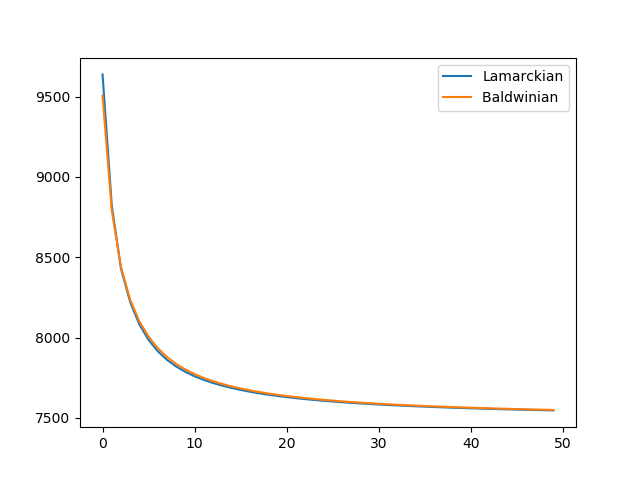
\includegraphics[width=0.9\textwidth]{hybrid_10.png}
	\end{figure}
	\begin{figure}[hbt!]
	\centering
	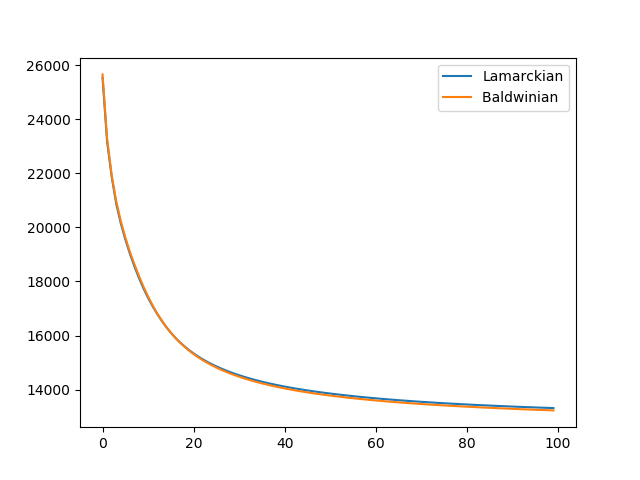
\includegraphics[width=0.9\textwidth]{hybrid_24.png}
	\end{figure}
\newpage

We can see that there is not a lot difference in the development of fitness in the two models. They also alternate which has the best fitness of the first generation. They both also end up pretty much at the same level of fitness after all generations are ran. To summarize the comparison between my GA and HA, the HA is a lot better for this optimization problem, where we are more concerned with effectiveness rather than efficiency. 

\end{document}